\documentclass{article}

% Recommended, but optional, packages for figures and better typesetting:
\usepackage{microtype}
\usepackage{graphicx}
\usepackage{subfigure}
\usepackage{booktabs} % for professional tables

\usepackage{mathtools}
\usepackage{physics}

% hyperref makes hyperlinks in the resulting PDF.
% If your build breaks (sometimes temporarily if a hyperlink spans a page)
% please comment out the following usepackage line and replace
% \usepackage{icml2020} with \usepackage[nohyperref]{icml2020} above.
\usepackage{hyperref}

% Attempt to make hyperref and algorithmic work together better:
\newcommand{\theHalgorithm}{\arabic{algorithm}}

% Use the following line for the initial blind version submitted for review:
% \usepackage{icml2020}

% If accepted, instead use the following line for the camera-ready submission:
\usepackage[accepted]{icml2020}

% The \icmltitle you define below is probably too long as a header.
% Therefore, a short form for the running title is supplied here:
\icmltitlerunning{Optimal flocking with a genetic algorithm}

\begin{document}

\twocolumn[
\icmltitle{Optimal boid flocking with a genetic algorithm}

% It is OKAY to include author information, even for blind
% submissions: the style file will automatically remove it for you
% unless you've provided the [accepted] option to the icml2020
% package.

% List of affiliations: The first argument should be a (short)
% identifier you will use later to specify author affiliations
% Academic affiliations should list Department, University, City, Region, Country
% Industry affiliations should list Company, City, Region, Country

% You can specify symbols, otherwise they are numbered in order.
% Ideally, you should not use this facility. Affiliations will be numbered
% in order of appearance and this is the preferred way.
% \icmlsetsymbol{equal}{*}

\begin{icmlauthorlist}
\icmlauthor{Frederik J. Mellbye}{to}
\end{icmlauthorlist}

\icmlaffiliation{to}{Institute for Computational and Mathematical Engineering, Stanford University, Stanford, USA}

\icmlcorrespondingauthor{Frederik J. Mellbye}{frederme@stanford.edu}

% You may provide any keywords that you
% find helpful for describing your paper; these are used to populate
% the "keywords" metadata in the PDF but will not be shown in the document
\icmlkeywords{Machine Learning, ICML}

\vskip 0.3in
]

% this must go after the closing bracket ] following \twocolumn[ ...

% This command actually creates the footnote in the first column
% listing the affiliations and the copyright notice.
% The command takes one argument, which is text to display at the start of the footnote.
% The \icmlEqualContribution command is standard text for equal contribution.
% Remove it (just {}) if you do not need this facility.

\printAffiliationsAndNotice{}  % leave blank if no need to mention equal contribution
% \printAffiliationsAndNotice{\icmlEqualContribution} % otherwise use the standard text.

\begin{abstract}
A genetic evolution-based approach is used to determine the coefficients of a boids model for optimal flocking. The model is inspired by the original Reynolds model, and adds predators. Predators chase the nearest boids, but flee if too many prey boids are flocked together. The results indicate that the coefficients tend to specific distributions, with a small gain in boid survival.
\end{abstract}

\section{Introduction}
\label{sec:introduction}
Boids, developed by Craig Reynolds in 1986 \cite{reynolds:1987:CG}, is an artificial life program that simulates flocking, herding and schooling behavour typically seen in animals in nature. The behavior of boids is governed by a set of simple rules, based on the proximity and heading of other nearby individuals.

Versions of the boids framework have been used in various applications, e.g. to generate realistic-looking flocks of flying animals and schooling fish. Examples are birds in the 1998 video game \textit{Half-Life}, and bat swarms in the 1992 feature film \textit{Batman Returns}. Versions of the boids framework have also been used in swarm robotics, for which flocking behaviour is often desired \cite{swarm}. In biology, the boids model has been important in understanding how schools of fish form and behave because of their close similarities \cite{reynolds:1987:CG}.

In the boids framework, each boid has a set of weights that prioritize the three behaviors of boids; cohesion, separation and alignment. To optimize the flocking behaviour of boids, a good set of parameters needs to be determined.

In this project, predators are added. Predators hunt down the nearest prey boid. If they get sufficiently close to a prey boid, the prey boid is eliminated from the simulation. To motivate flocking, the notion of group defense is added: In sufficiently large flocks prey boids are able to fend off attackers. This is implemented as a steering force on predators. Within this framework many generations of a genetic algorithm is employed to optimize flocking.

\section{Background}
\label{sec:background}
Boid implementations commonly use a heuristic technique to determine the coefficients, through visualizations of the boid system. The coefficients were chosen for different behaviors, such as matching behaviour seen in nature for movies \cite{reynolds:1987:CG}.

Optimization approaches have also been used. Different approaches include maximizing the total aligntment or minimizing the avarage distance between boids. Particle swarm and genetic optimization techniques have been applied to optimize for this behavior \cite{ntnu}.

\section{Approach}
\label{sec:approach}
\subsection{Boids system}
The boids system has many parameters, these are summarized in Table~\ref{tbl:params}.
\subsubsection{Steering forces}
\begin{figure*}
  \centering
  \includegraphics[width=.25\linewidth]{images/separation.png}
  \includegraphics[width=.25\linewidth]{images/alignment.png}
  \includegraphics[width=.25\linewidth]{images/cohesion.png}
  \caption{Steering forces on prey boids. From the left: Separation, alignment and cohesion \cite{reynolds:1987:CG}.}
  \label{fig:preyforces}
\end{figure*}

Prey boids have the three original steering forces; cohesion, separation and alignment \cite{reynolds:1987:CG}. These are depicted in Figure~\ref{fig:preyforces}.

The cohesion force $F_c$ on boid $b_j$ is given by
\begin{align}
  F_c = c_c \frac{1}{n-1} \sum_{i \neq j}^{n} x_i - x_j
\end{align}
where $c_c$ is a corresponding coefficient on the force, and $x_i$ is the position of $b_i$. It draws boids closer to the general position of neighboring boids.

Similarly, the separation force is given by
\begin{align}
  F_s = c_s \frac{1}{n-1} \sum_{i \neq j}^{n} \frac{x_i - x_j}{\norm{x_i - x_j}_2}
\end{align}
This force only considers boids that are very close, and ensures boids do not fly too close to each other. In some sense this simulates that the boids have some size and avoid crashing.

Finally, the alignment force is
\begin{align}
  F_a = c_a \frac{1}{n-1} \sum_{i \neq j}^{n} v_i - v_j
\end{align}
where $v_i$ is the velocity vector of $b_i$. Boids steer towards the average heading of neighboring boids.

The forces are combined to produce a total force, which is clipped, simulating how animals only can turn at certain rates. The total force is therefore given by
\begin{align*}
  F = \max(F_c + F_s + F_a, F_\text{max})
\end{align*}
The boid masses are normalized, so the force is equal to the acceleration. We also have a time step $\Delta t = 1$. Therefore, the velocity and position updates are
\begin{align*}
  v^{(k+1)} &= v^{(k)} + F \\
  x^{(k+1)} &= x^{(k)} + \frac{v^{(k+1)}}{\norm{v^{(k+1)}}_2}
\end{align*}
Note that the velocity is normalized. This paper assumes that all boids fly at their max speed $v_\text{max}$ at all times.

Predators follow three forces; they hunt the nearest prey boid, flee from prey boids if too many prey boids are present (simulating how prey animals often are able to fend of predators when grouped together) and separation. These added forces are depicted in Figure~\ref{fig:predatorforces}.

Let $x$ denote the position of a particular predator, and $x_i$ the position of the prey boids for $i = 1,\hdots,N$. The hunting force $F_h$ is simply a unit vector towards the nearest prey. The direction is:
\begin{align}
  F_h = x - \arg \min_{x_i} \norm{x_i - x}_2
\end{align}

The tendency of predators to flee when too many prey boids are close together is given by the force $F_f$. The force is only applied if at least 3 prey boids are within a distance of 80 from the target. Let $x_t$ denote the position of the current target of

\begin{figure*}
  \centering
  \includegraphics[width=.25\linewidth]{images/chase.png}
  \includegraphics[width=.25\linewidth]{images/avoid.png}
  \caption{Hunt and flee steering forces on predator boids. Modified versions of images from \cite{reynolds:1987:CG}.}
  \label{fig:predatorforces}
\end{figure*}

\subsubsection{Initialization}
In each simulation, the boids $b_i$ have randomly initialized positions and velocities. Let $w$ and $h$ denote the system width and height respectively. The positions are sampled uniformly, i.e.
\begin{align*}
  x_i \sim \begin{bmatrix} u(0.2w, 0.5w) \\ u(0.2h, 0.8h) \end{bmatrix}
\end{align*}
where $u(a,b)$ denotes a uniform random variable on $[a,b]$. This way prey boids spawn on the left half of the environment. Predators similarly spawn on the other half. This attempts to ensure that prey boids are not killed immediately before they have the chance to flock.

The velocities are set to
\begin{align*}
  v_i \sim \begin{bmatrix} 1 \\ u(0,1) \end{bmatrix}
\end{align*}
i.e. towards the center with some random $y$-component.

\subsection{Genetic algorithm}
The goal of this project is to determine the set of coefficients of an entire flock of prey boids that maximizes their survival in the presence of predators. The design is the set of coefficients of all boids $\{c_i\}_{i=1}^{n}$. A genetic algorithm is employed to optimize these coefficients for survival, which is acheived when the boids are better at flocking.

Genetic algorithm approaches commonly repeat three components; selection, crossover and mutation \cite{kochenderfer}. The fashion in which these are performed commonly differs based on the particular application and the way the chromosomes are encoded.

\subsubsection{Selection}
In each simulation, a subset of the prey boids survive through the simulation. In this project, the selection step simply selects the survivors of each generation. This is motivated from the principle of natural selection.

\subsubsection{Crossover}
Crossover is performed as follows: For each new boid, for each coefficient,
the new boid gets one of the parents values with uniform probability. This way, traits that predict survival are propagated from one generation to the next.

\subsubsection{Mutation}
To introduce the possibility of new variations, mutations are sporadically added in the form of gaussian noise. With probability $p_m$, we add $\mathcal{N}(0, \sigma^2)$ noise to a particular coefficient of a new boid. The variance is tuned such that a shift in coefficient values is seen over many generations.

\begin{table*}
  \centering
  \caption{Parameters used for the genetic algorithm and boids simulation. Most of these were tuned heuristically.}
  \label{tbl:params}
\begin{tabular}{*4l} \toprule
\emph{Name}       & \emph{Symbol} & \emph{Value} & \emph{Description} \\ \midrule
System width  & $w$ & 3360  & \\
System height & $h$ & 2100 & \\
Number of prey boids & & 200 & Number of prey boids in each simulation \\
Number of predators & & 10 & Number of predators in each simulation \\
Iterations & & 8000 & Iterations in each simulation \\
Mutation probability& $p_m$ & 0.1 & Probability of mutation for a particular coefficient \\
Mutation spread        &  $\sigma$      & 0.1  & Standard deviation of mutations   \\
Separation range           &        &  & Distance within which the separation force is applied   \\
Prey force ranges         &        &  2000 & Distance within which alignment and cohesion forces are applied \\
Kill range          &        & 4.0  & Range from which predators kill prey \\
Hunting coefficient & $c_h$ &   1.0   & \\
Number of neighbors & & 3 & Number of neighbors required for group defense \\
Flee distance & & 80 & Maximal distance of neighbors for group defense \\
Predator $v_\text{max}$ &       & 1.1     & Predator velocity \\
Prey $v_\text{max}$ &        & 1.0     & Prey velocity \\
Predator max force & $F_\text{max, predator}$ & 0.1& \\
Prey max force & $F_\text{max, prey}$ & 0.04 & \\
Separation initial distribution& & $u(0,3)$ & \\
Alignment initial distribution & & $u(0, 0.5)$ & \\
Cohesion initial distribution & & $u(0, 0.5)$ & \\\bottomrule
\end{tabular}
\end{table*}

\subsection{Computational considerations}
For performance reasons, the implementation of the boids framework and genetric algorithm was done in C++.

With a naive implementation the computation of the steering forces is $\mathcal{O}(n^2)$. For each boid, the positions of all other boids are required. This is clearly not feasible for simulations with many boids and many generations of evolution.

To reduce the computational load, each boid locally keeps track of it s nearest neighbors and only use these to compute steering. This allows constant time lookup of neighbors, which greatly simplifies the complexity, at the cost of the small error introduced by the approximation. The list of neighbors is updated with a particular frequency, for this project every 10 time steps.

\section{Results}
\label{sec:results}
Figures~\ref{fig:survival} and~\ref{fig:coeffs} show the number of survivors and coefficient statistics over the course of 300 generations of evolution.

The figures show a slight, but very noisy increase in the average number of survivors. This could indicate that there is a slight increase in the rate of survival. The average coefficient values flatten out with slighly decreasing standard deviations.

\begin{figure}
  \centering
  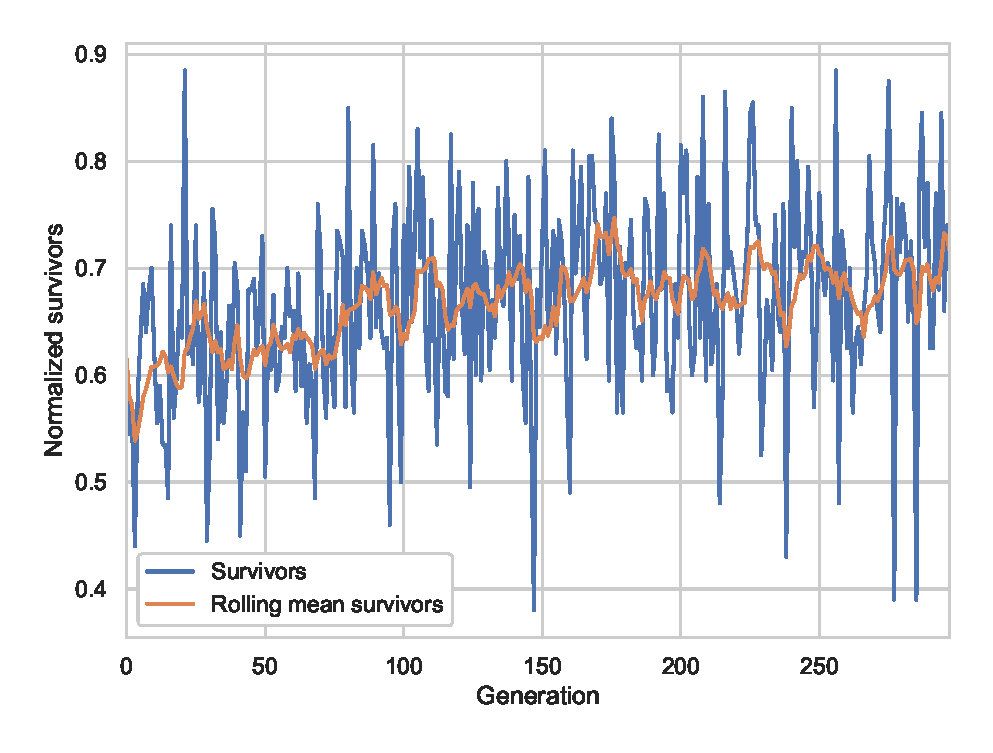
\includegraphics[width=\linewidth]{figures/survival.eps}
  \caption{Proportion of boids that survive each generation. The orange line shows the mean of the last 10 numbers of survivors. It is clear that there is high randomness in the number of survivors, likely due to the inherent randomness of each simulation. A lot of boids do not have time to move towards other flockmates before a predator reaches them.}
  \label{fig:survival}
\end{figure}

\begin{figure}
  \centering
  \includegraphics[width=\linewidth]{figures/coeffs.pdf}
  \caption{Mean coefficient value across all boids of each particular generation. The shaded regions show the standard deviations of the coefficients.}
  \label{fig:coeffs}
\end{figure}

\section{Conclusion}
\label{sec:conclusion}
As can be seen from the number of survivors in Figure~\ref{fig:survival}, there is a lot of randomness in the objective. This is likely due to the random initialization of boids, where in some cases the boids are initially more scattered and easy targets for the predators. In other cases the boids may have a better initialization for early flocking, which leads to more survivors.

Despite the large fluctuations in survivors, which is almost indistinguishable from noise, Figure~\ref{fig:coeffs} shows the coefficients tend towards specific values. The standard deviation of each coefficient is decreasing, indicating that the boids get more and more similar coefficient values closer to the mean.

\section{Future directions}
\label{sec:future}
The results are quite unreliable due to the large degree of randomness in the objective function. Future work should therefore explore ways to reduce the randomness of the simulations, in particular through exploring other initialization strategies. Further exploration of other simulation parameters such as the system size, force range and max forces may also help reduce the randomness.

This project made some simplifications to the physics of the simulations. For applications such as drone swarms a more realistic physics simulation is neccesary, with proper forces and masses.

Future work could also explore the effect of adding obstacles that the boids have to avoid.

Several modifications are possible to make the boids simulations more computationally efficient. Computing the forces of the boids can be done in parallel, the space can be partitioned into sections for faster lookup of nearby boids (this was done in the project using a QuadTree).


% In the unusual situation where you want a paper to appear in the
% references without citing it in the main text, use \nocite

\bibliography{references}
\bibliographystyle{icml2020}

%%%%%%%%%%%%%%%%%%%%%%%%%%%%%%%%%%%%%%%%%%%%%%%%%%%%%%%%%%%%%%%%%%%%%%%%%%%%%%%
%%%%%%%%%%%%%%%%%%%%%%%%%%%%%%%%%%%%%%%%%%%%%%%%%%%%%%%%%%%%%%%%%%%%%%%%%%%%%%%


\end{document}


% This document was modified from the file originally made available by
% Pat Langley and Andrea Danyluk for ICML-2K. This version was created
% by Iain Murray in 2018, and modified by Alexandre Bouchard in
% 2019 and 2020. Previous contributors include Dan Roy, Lise Getoor and Tobias
% Scheffer, which was slightly modified from the 2010 version by
% Thorsten Joachims & Johannes Fuernkranz, slightly modified from the
% 2009 version by Kiri Wagstaff and Sam Roweis's 2008 version, which is
% slightly modified from Prasad Tadepalli's 2007 version which is a
% lightly changed version of the previous year's version by Andrew
% Moore, which was in turn edited from those of Kristian Kersting and
% Codrina Lauth. Alex Smola contributed to the algorithmic style files.
